\section{Implementation}
This section provides a comprehensive overview of the system's implementation. It includes the user interface illustrating each component and feature implemented in our email marketing tool during the third sprint. The user interface was designed to be simple and user-friendly. The goal was to make the tool easy to use even for users without much technical expertise.

\subsection{Insights Dashboard}

\paragraph*{Tracking Mechanism:}
To gather data for the Insights Dashboard, we rely on a tracking system. When an email campaign is sent, each email contains unique identifiers (Message ID). As recipients interact with the emails (e.g., open an email, click a link), these identifiers trigger events. Our system captures these events and records them in our database.

\paragraph*{Brevo Transactional Webhook:}

We've integrated Brevo's transactional webhook into our system. When specific events occur (e.g., email opened, link clicked), Brevo sends HTTP requests to our server. Our Email Service processes these requests, extracts relevant data (such as recipient email, campaign ID, event type), and updates our database. Real-time updates ensure that the Insights Dashboard reflects the latest campaign performance.

\begin{figure}[ht]
	\centering
	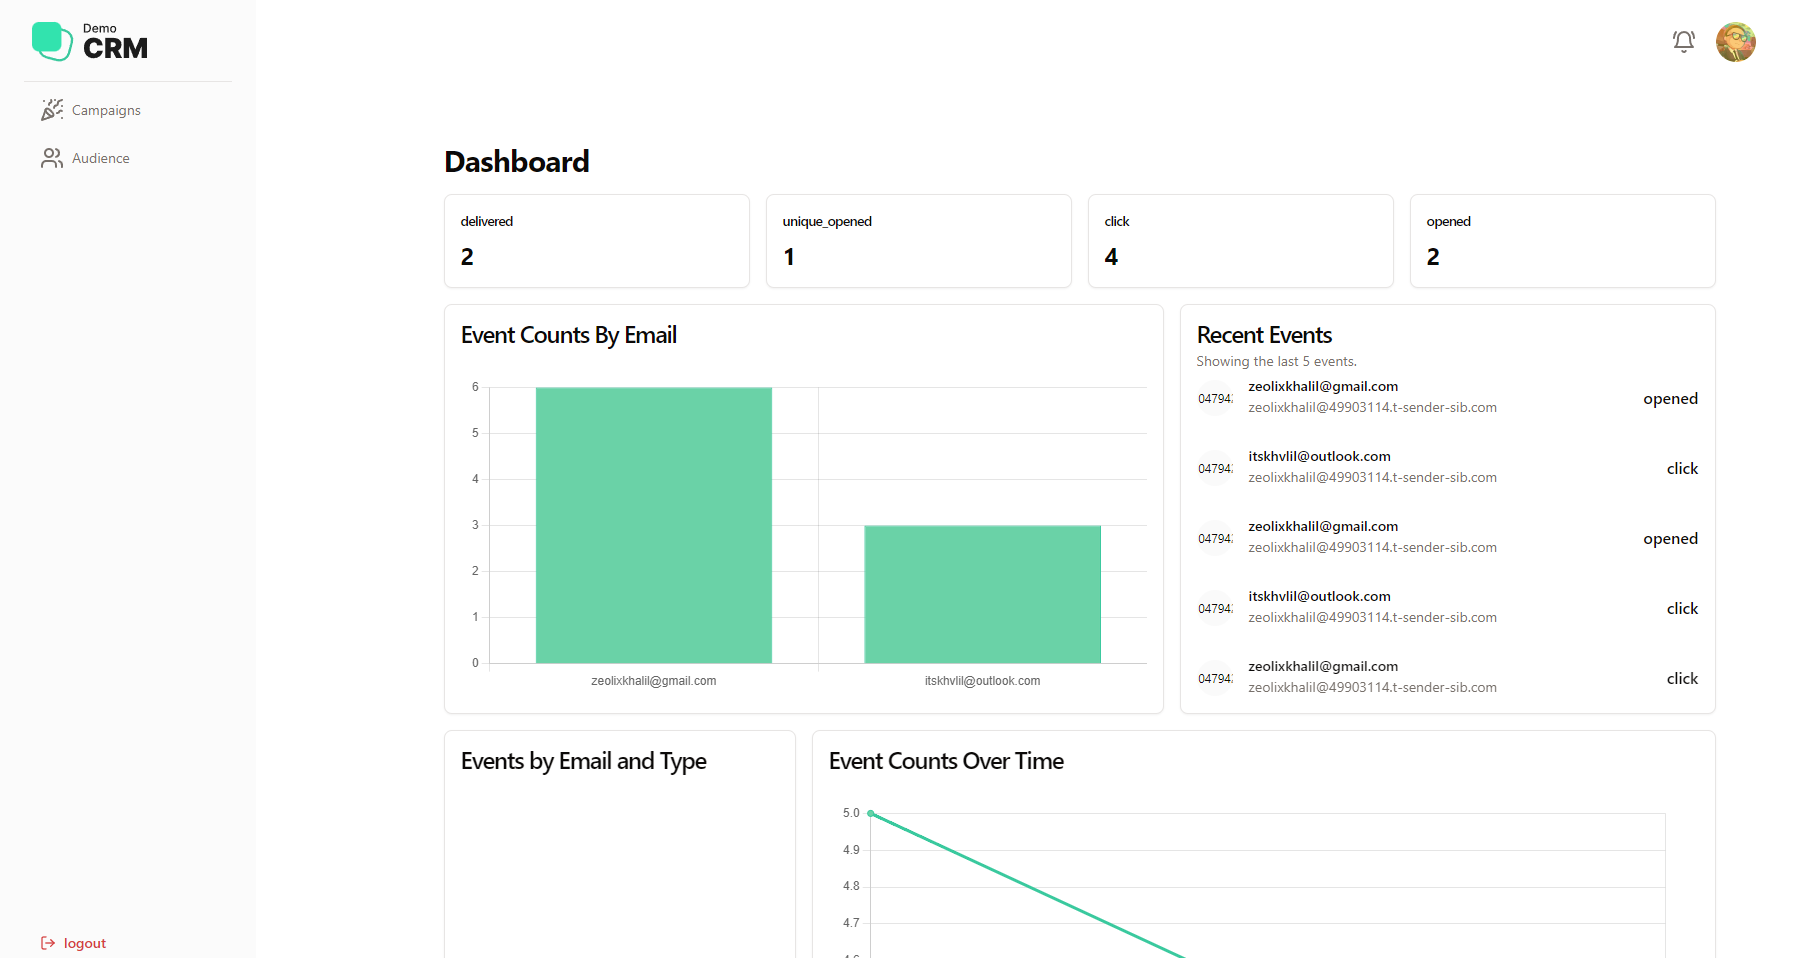
\includegraphics[width=\linewidth]{Images/Sprint3/Screenshot 2024-06-04 002816.png}
	\caption{User Interface for Campaigns Dashboard}
	\label{fig:User Interface for Campaigns Dashboard}
\end{figure}